\section{Implementation} \label{sec:impl}
In this section, we will describe the implementation of our protype in detail. First, we will outline the used framework and tools in each application stack. Then, we will describe our development setup using Ethereum test network. Furthermore, we will describe the implementation of the core data structures and smart contracts. And finally, we will explain the secured transaction flow without a need for a trusted third-party.

\subsection{Architecture}
Our technology stack is illustrated in Figure~\ref{fig:techstack}. For the web front-end we used the popular setup containing React~\cite{React}, Webpack~\cite{Webpack} and Redux~\cite{Redux} using JavaScript as the primary programming language. The smart contracts are written in Solidity. Additionally, we utilized various tools such as Truffle~\cite{Truffle}, a widely-used development framework for Ethereum. Although Truffle allows us to run a local Ethereum testnet, Ganache~\cite{Ganache} came in very handy since it offered an user interface, where we could inspect the current state of the ledger including all performed transactions. Additionally, we used OpenZeppelin~\cite{OpenZeppelin}, a framework containing reusable smart contracts (e.g. access control, ERC-20, ERC-721, ...) that have been tested and reviewed by the Ethereum community. As for the backend, we went with Node.js using ExpressJS as the underlying web-framework along with MongoDB to persist meta-data of car assets and sales.

\begin{figure}[htbp]
\centerline{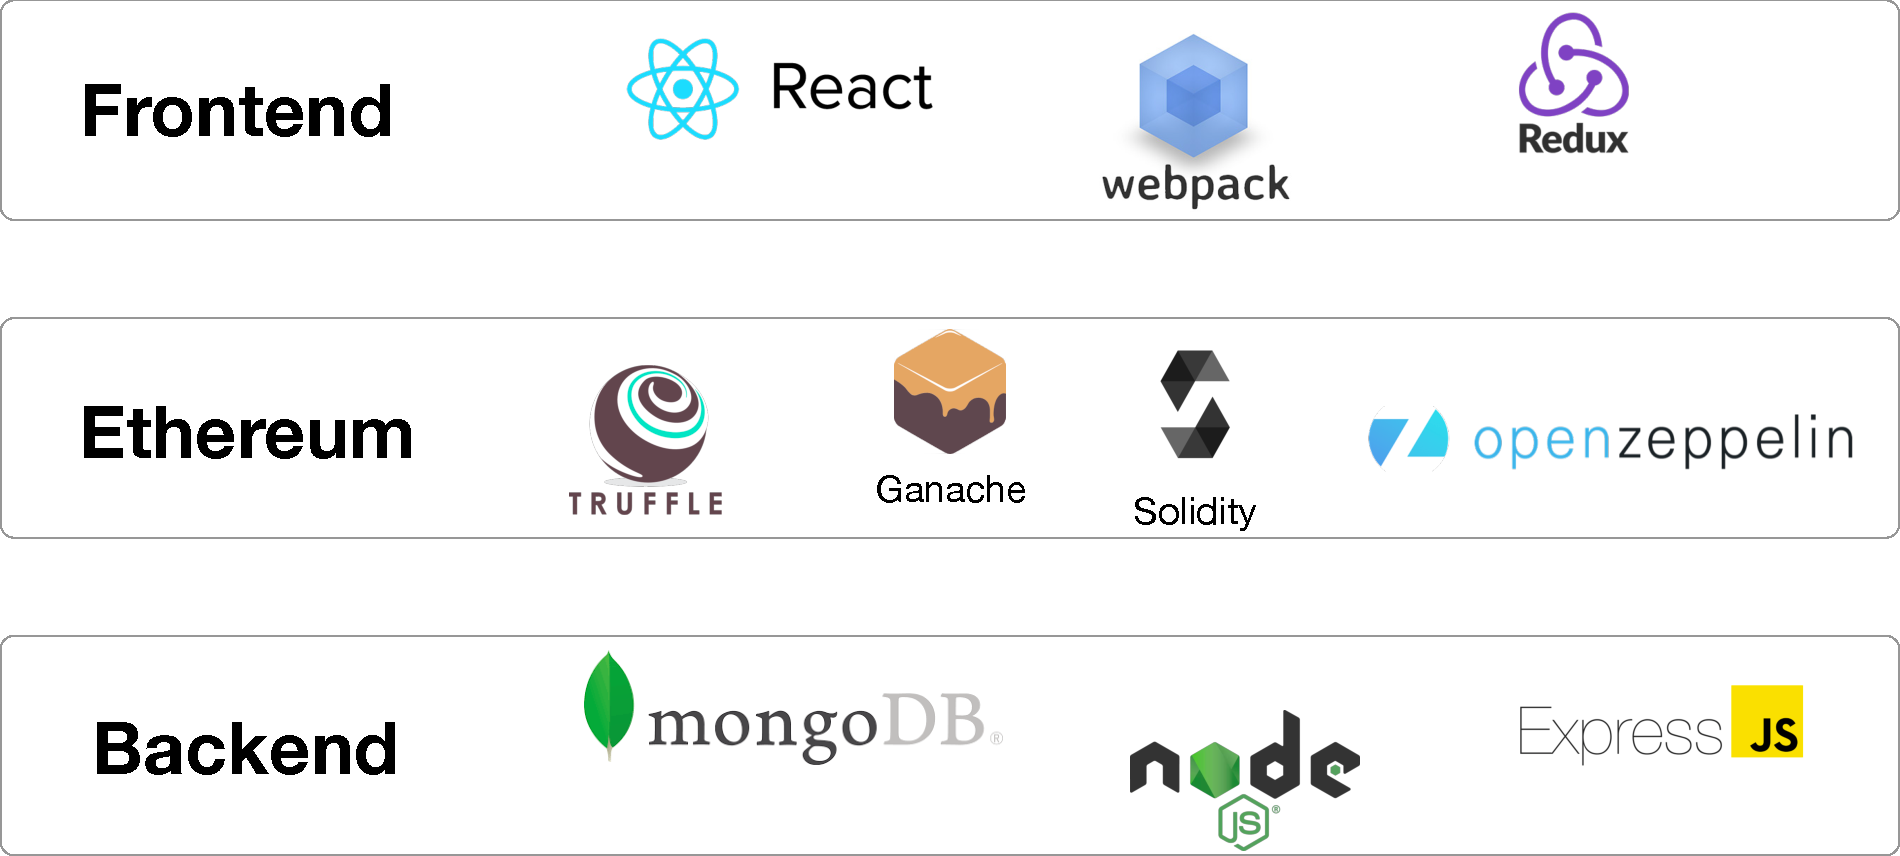
\includegraphics[width=0.9\textwidth]{figures/tech_stack.pdf}}
\caption{Technology stack \label{fig:techstack}}
\end{figure}

\subsection{Ethereum Test Network}
For deploying and testing our smart contracts, we used a personal blockchain which only runs on our system and does not interact with the main Ethereum network. Truffle's command line interface allows such setup which comes with ten Ethereum wallets containing 100 Ether each. This allows us to test smart contracts freely without paying real fees. An alternative would be deploying the smart contracts to one of the many testnets (e.g. Rinkeby~\cite{Rinkeby}) which allows a better testing of the real world performance. This is especially useful when nearing production stage, however before that, we found it to be too inconvenient, tedious which slows down the development tremendously.

\subsection{Data Structures}
In order to store car assets and make them temper-proof, we had to define the corresponding data structures that are stored and managed directly on the Ethereum ledger. The struct as shown in Listing~\ref{lst:car_struct} represents a car, it contains only the most important attributes such as manufacturer, mileage and accidents count. Note that we decided against storing additional attributes, because persisting large amount of data on Ethereum can be very costly and could lead to blockchain bloating~\cite{BlockchainBloating}. Instead, non-critical information (e.g. horse power, images) are stored in our back-end database. Since cars are not removable, they are all stored in an growing array, where the array index also serves as the car identifier. Sale structures also only contain the most important information: seller, bidder, price of the car and time when the sale has started (see Listing~\ref{lst:sale_struct}). Unlike cars, sales are stored inside a mapping with the asset identifer as the key value. This allows the deletion of a sale after it has been finished.

\begin{minipage}[t]{0.45\linewidth}
\begin{lstlisting}[caption={Car struct}, language=Solidity, label=lst:car_struct, numbers=none]
struct Car {

  // The timestamp of car creation.
  uint64 creationTime;

  // The ID of the car manufacturer
  uint256 manufacturerId;

  // The ID of the car model
  uint16 modelId;

  // The mileage of the car (in km)
  uint32 mileage;

  // Number of accidents involving this car
  uint8 accidentsCount;
}
\end{lstlisting}
\end{minipage}
\hspace{10mm}
\begin{minipage}[t]{0.45\linewidth}
\begin{lstlisting}[caption={Sale struct}, language=Solidity, label=lst:sale_struct, numbers=none]
struct Sale {
  // Current car owner
  address seller;
  // Person who has bid on this sale
  address bidder;
  // Car Price
  uint128 price;
  // Time when sale started
  uint64 startedAt;
}
\end{lstlisting}
\end{minipage}

\clearpage

\subsection{Smart Contracts}
An overview of the smart contracts is shown in Figure~\ref{fig:class_diagram}.
We split the various functionalities in different contracts and used inheritance to combine them meaningfully. Effectively, the application consists of two main contracts which we will describe in the following more in detail.

\subsubsection{Access Control}
As mentioned in our concept (see Section ~\ref{sec:concept}), the creation and update of cars is only permitted to car manufacturers. Therefor, we implemented an access control mechanism, which contains the following two roles:
  \begin{enumerate}
    \item \textbf{Administrator}: can add or remove manufacturers
    \item \textbf{Manufacturer}: can initially create car assets and update car statistics (e.g. mileage)
  \end{enumerate}
To achieve this, our implementation inherits from OpenZeppelin's role-based access control (RBAC) smart contracts~\cite{OpenZeppelinGithub}.

\subsubsection{Car}
The \textit{RideBase} contract serves as the foundation for our DApp, it holds all common structs, events and variables. In particular, it defines the array containing all car structs and a mapping of car identifiers to their owners. Additionally, it holds a reference to our market contract, allowing the interaction with it. This reference can be updated after deployment so that we can replace the market contract in case something goes wrong. The \textit{RideCore} contract is the main interface for interacting with our DApp, is handles creating, updating and tracking the current status of cars.

\subsubsection{Ownership}
Tracking and transferring the ownership of an asset is a well-known use case in blockchain technology. Fortunately, the ERC-721 Non-Fungible Token Standard~\cite{ERC721Summary} provides a solution for this (see also Section~\ref{sec:ERC721}). Non-fungible tokens (NFTs) can represent ownership over digital or physical assets such as houses, collectable cards but also cars. NFTs are unique, distinguishable and are thus not interchangeable. The \textit{RideOwnership} contract, from which our main car contract inherits from, implements the ERC-721 interface. By utilizing the mapping from asset identifier to owner address, we can always ensure the correctness of asset ownership and transfer.

\subsubsection{Market}
Our market implementation consists of two contracts. The first is \textit{MarketBase} which contains all structs, events, and internal methods for managing sales. In particular, it holds a mapping of assets to their corresponding sale structs and a reference to the ERC-271 implementation to perform ownership transfers. The second contract is \textit{MarketCore} which inherits from \textit{MarketBase} and provides the main interface for interacting with the sales. It handles operations such as creating sales, tracking the current status of sales, bidding on sales, confirming or rejecting sales.

\subsection{Transaction Flow}
In order to make the transaction between buyer and seller trustless and secure, we implemented an escrow mechanism which should simulate the intermediary third-party. Only upon certain conditions, the ownership transfer is performed. In the first iteration, we implemented the transaction process like the following:
\begin{enumerate}
  \item \textbf{Sell}: Seller defines a price and puts a car on sale. I.e. car asset is transferred to our market contract.
  \item \textbf{Buy}: Buyer pays the requested price, the money goes to our market contract.
  \item \textbf{Escrow}: Car is transferred to buyer and the money is transferred to seller simultaneously.
\end{enumerate}

Although this approach works in theory, there are several flaws that made us rethink the whole process. Firstly, the seller cannot really decide to whom the car is sold, since it is basically first come, first served. Secondly, once the transaction is performed, there is no way for the buyer to cancel his order, since it automatically goes through if the requested price was paid. For this particular reasons, we updated the flow and added an extra confirmation step.

\begin{enumerate}
    \item \textbf{Sell}: Seller defines a price and puts a car on sale. I.e. car asset is transferred to our market contract.
    \item \textbf{Bid}: Buyer bids on car and pays the requested price upfront, the money goes to our market contract. Car is now reserved, meaning no other person can place a new bid on it.
    \item \textbf{Confirm}: Buyer and seller both now have the option to cancel the bid, thus returning the money back to the buyer and make the car available again. Seller has additional option to confirm the bid which triggers the asset transfer.
    \item \textbf{Escrow}: If confirmed, car is transferred to buyer and the money is transferred to seller simultaneously.
  \end{enumerate}

This extra step should mitigate human errors and give buyer and seller more room for action. In addition to that, it improves the resemblance to the real world process of buying a car.

\begin{figure}[htbp]
\centerline{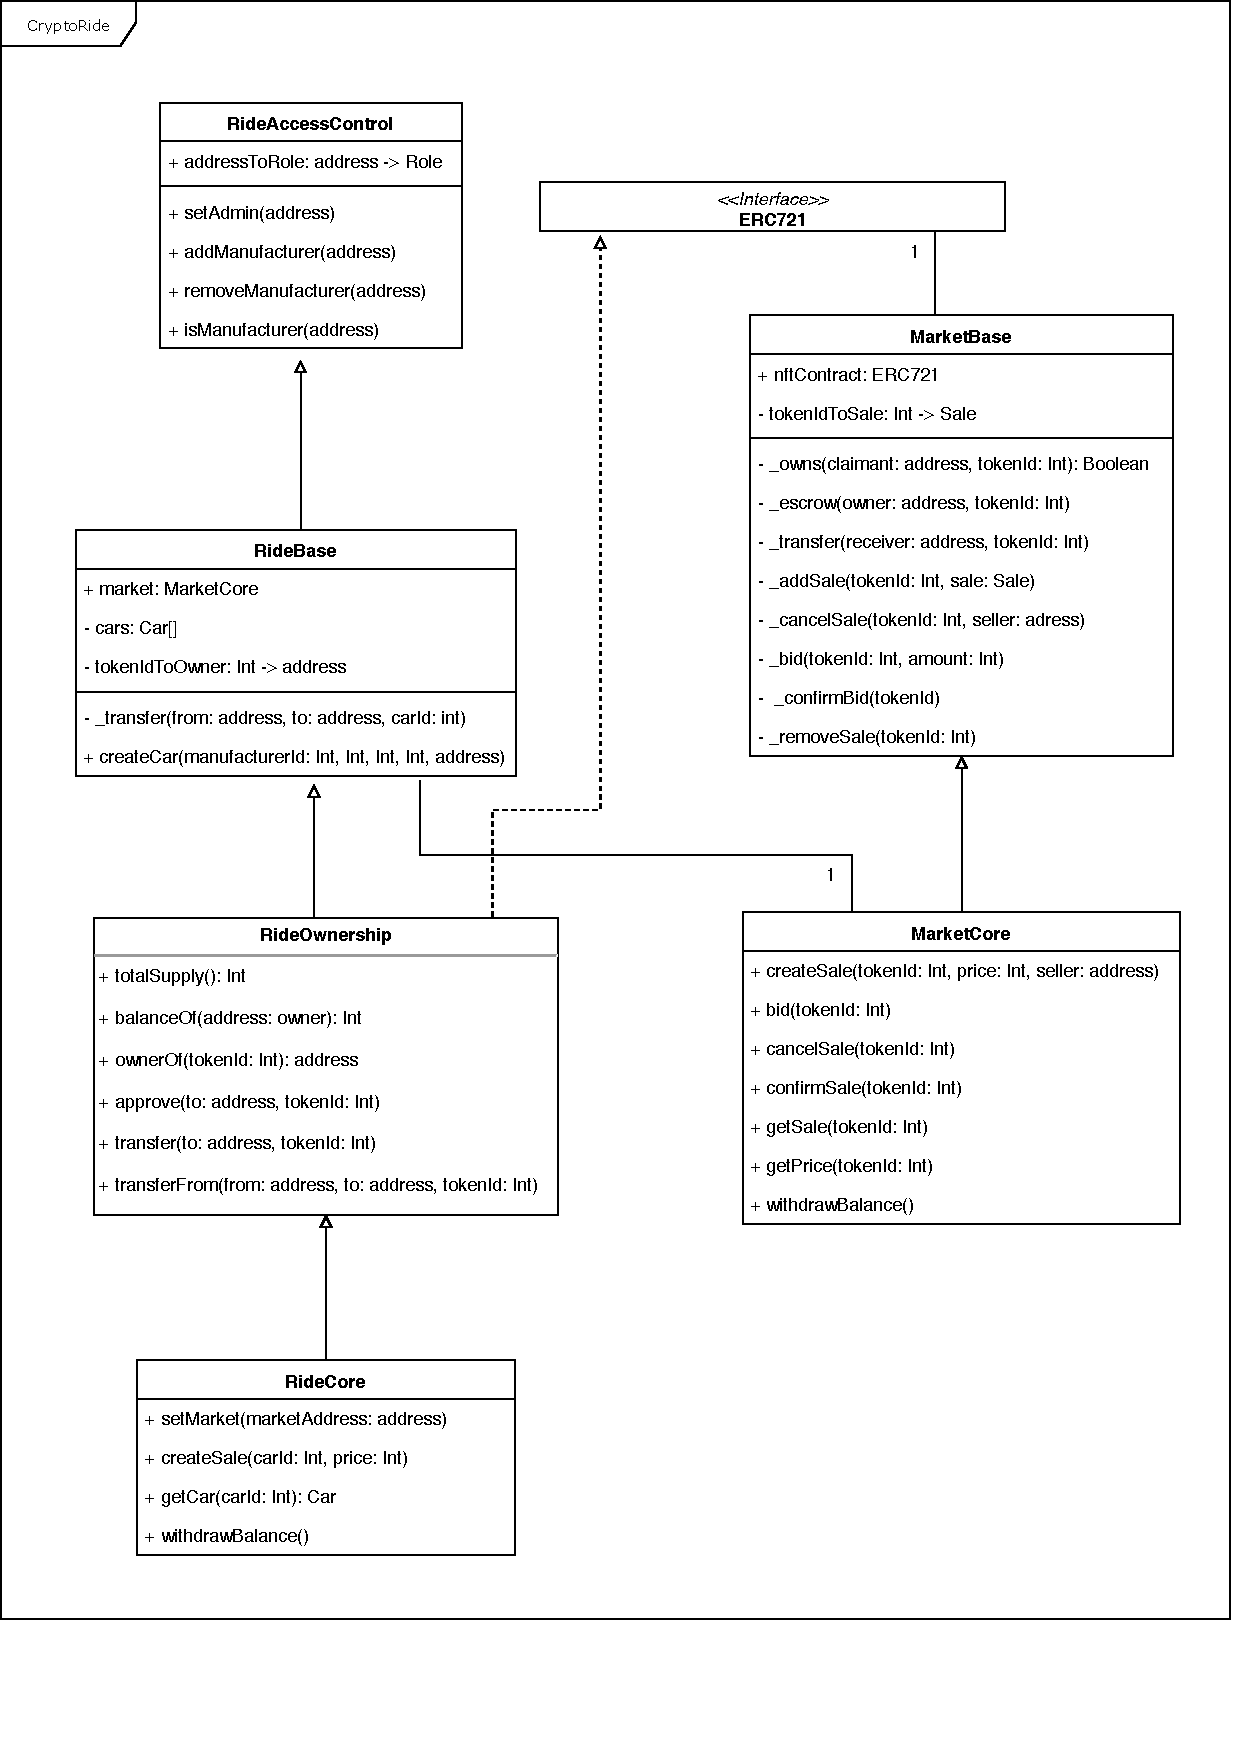
\includegraphics[width=\textwidth,height=\textheight,keepaspectratio]{figures/smart_contracts_uml.pdf}}
\caption{Overview: Smart Contracts \label{fig:class_diagram}}
\end{figure}


% \subsubsection{Testing}
% In order to verify the correctness and functional behavior of our smart contracts, we implemented automated tests, which should simulate the user interactions with our application (e.g. creating a car, selling and buying a car, etc.). The tests are written in Solidity or JavaScript and are executed using Truffle's command line interface~\cite{TruffleTest}.

\clearpage

\subsection{MetaMask}
MetaMask~\cite{MetaMask} is an extension which allows users to interact with the Ethereum network directly from the browser. It serves as our main tool for the secure user authentication and car asset transfer. By injecting the Ethereum web3 API into every website's JavaScript context, DApps can read from the blockchain through MetaMask. Furthermore, it lets users create and manage their identities, i.e. when a DApp wants to perform a transaction, the user is notified with a secure interface for reviewing the transaction before accepting or rejecting it (see Figure~\ref{fig:metamask_transaction}). In order to interact with our application, the MetaMask browser extension has to be installed either on Google Chrome or Mozilla Firefox.

\begin{figure}[htb]
  \centering
  \begin{subfigure}{.4\textwidth}
    \centering
    \fbox{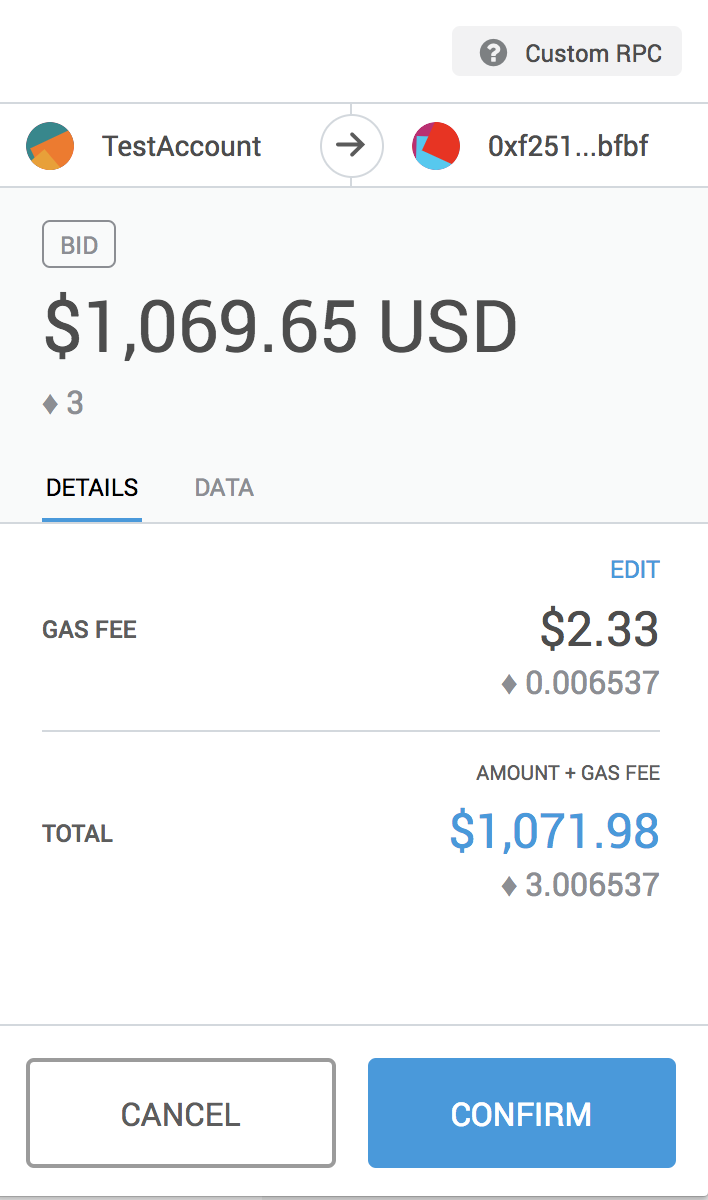
\includegraphics[width=0.9\linewidth]{figures/cryptoride_screens/metamask_transaction.png}}
    \caption{Transaction \label{fig:metamask_transaction}}
  \end{subfigure}
  \hspace{10mm}
  \begin{subfigure}{.4\textwidth}
    \centering
    \fbox{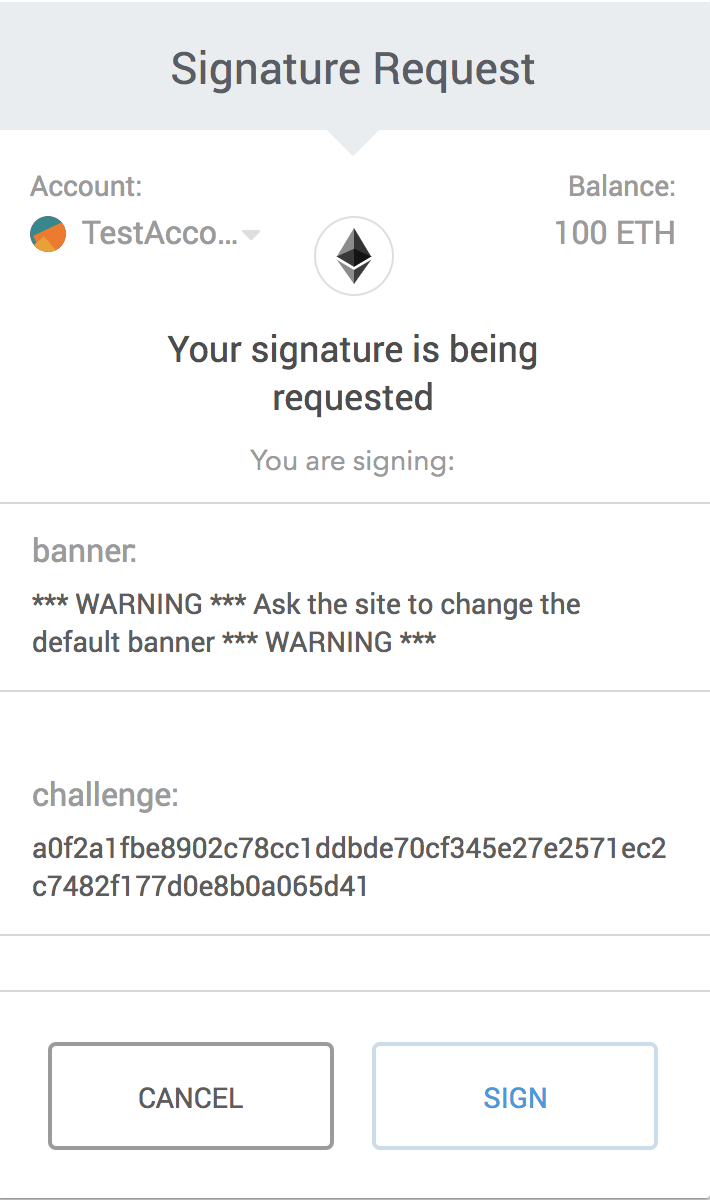
\includegraphics[width=0.9\linewidth]{figures/cryptoride_screens/metamask_sign.png}}
    \caption{Signing \label{fig:metamask_signing}}
  \end{subfigure}
  \caption{MetaMask}
\end{figure}


% \subsection{Application Flow}
% A rough overview of the application flow is illustrated in Figure~\ref{fig:application_flow}. In order to use our platform, an account is needed. This can be done by registrating with a valid Ethereum account and having MetaMask installed on the browser. When logged in, the user can look for active sales or putting a car on sale. Manufacturers addresses are recognized by the front-end, they are permitted to create new car assets.

\subsubsection{Authentication}
We use MetaMask for handling user authentication over the traditional username and password login. This approach only requires an Ethereum account and no personal identifying information.
First, the user is asked to sign a challenge using his private key (see Figure~\ref{fig:metamask_signing}). Then, the generated signature is then sent to the back-end for validation. Finally, upon success, the backend will respond with a JSON Web Token (JWT) which authenticates the user. This token can also be stored for the current session.

% \begin{figure}[htbp]
% \centerline{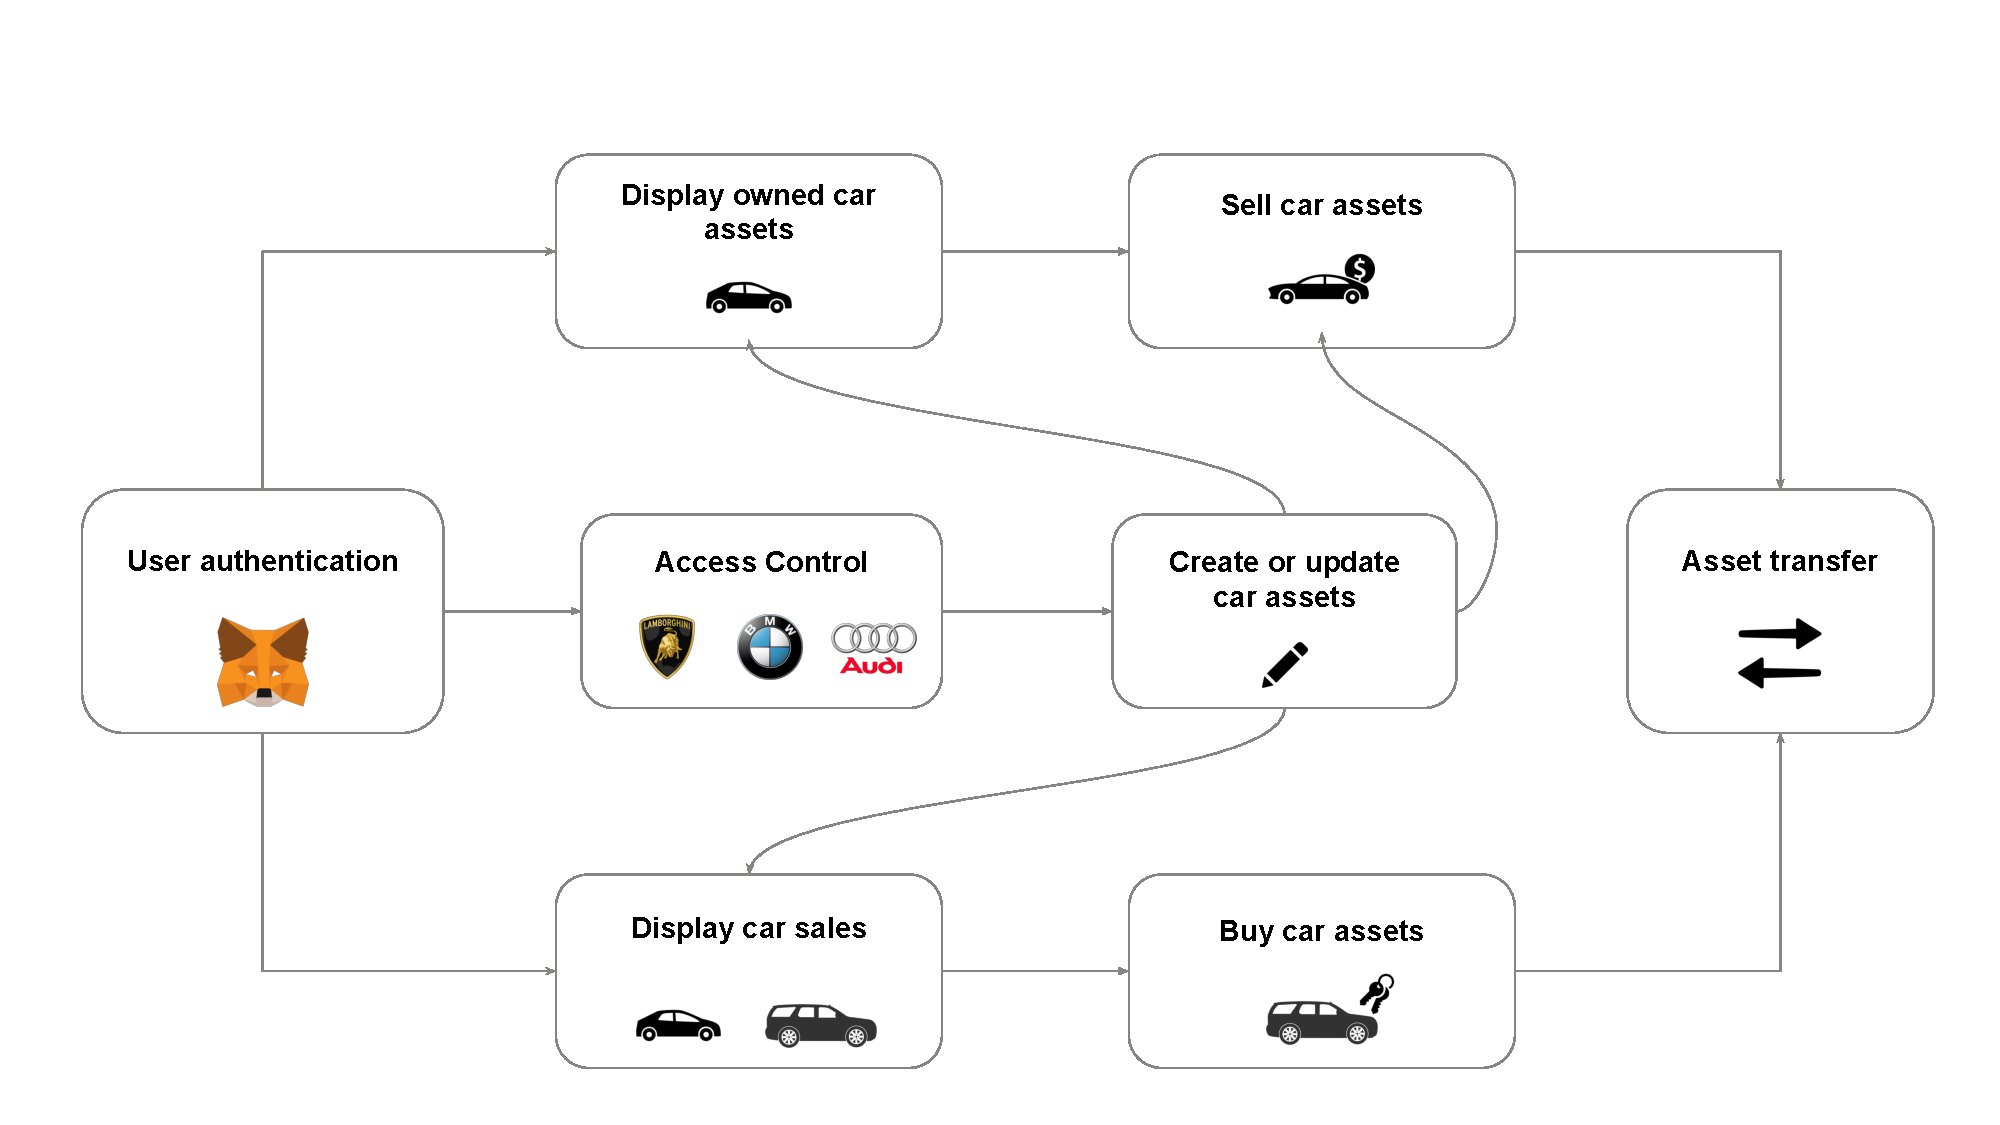
\includegraphics[width=0.9\textwidth]{figures/application_flow.pdf}}
% \caption{Application Flow \label{fig:application_flow}}
% \end{figure}



% \subsection{Screenshots}
% \begin{figure}[htbp]
% \centerline{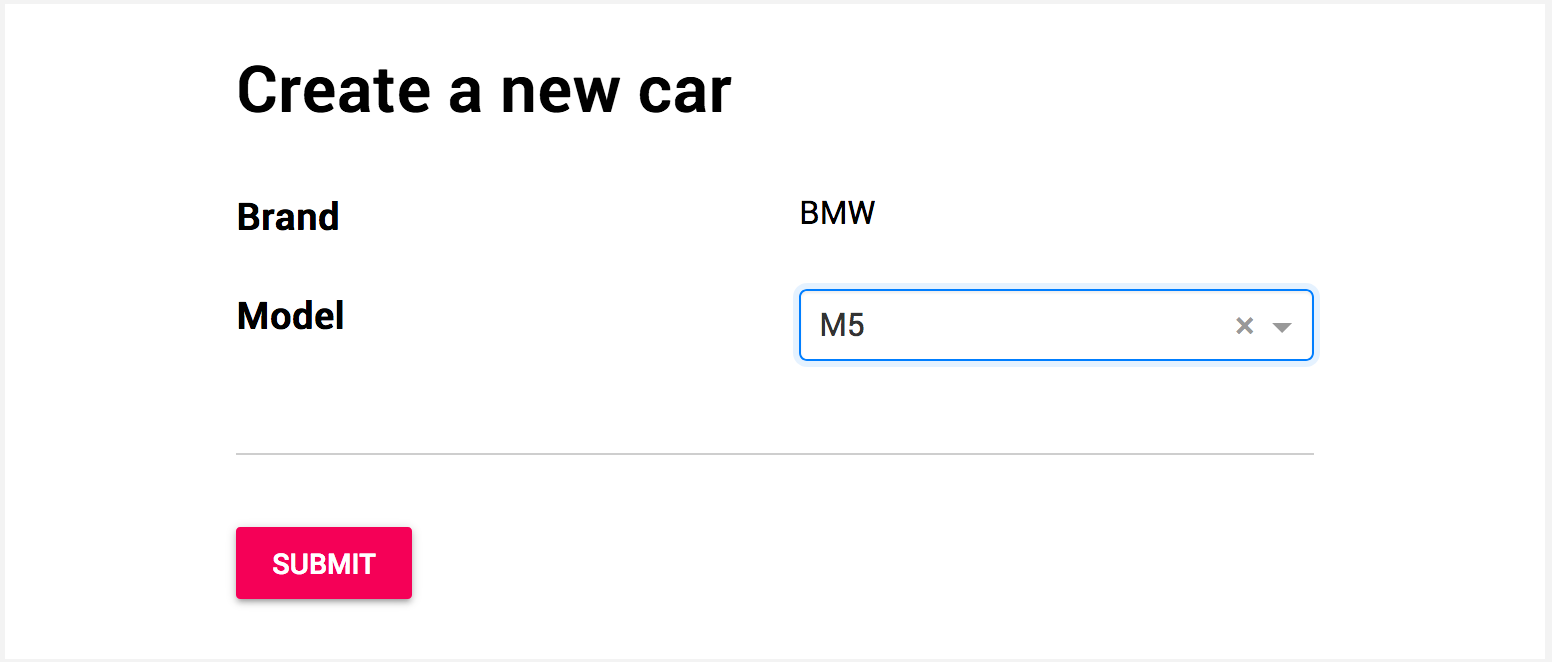
\includegraphics[width=1\textwidth]{figures/cryptoride_screens/create_car.png}}
% \caption{Screen: Create Car \label{fig:screen_create_car}}
% \end{figure}
%
% \begin{figure}[htbp]
% \centerline{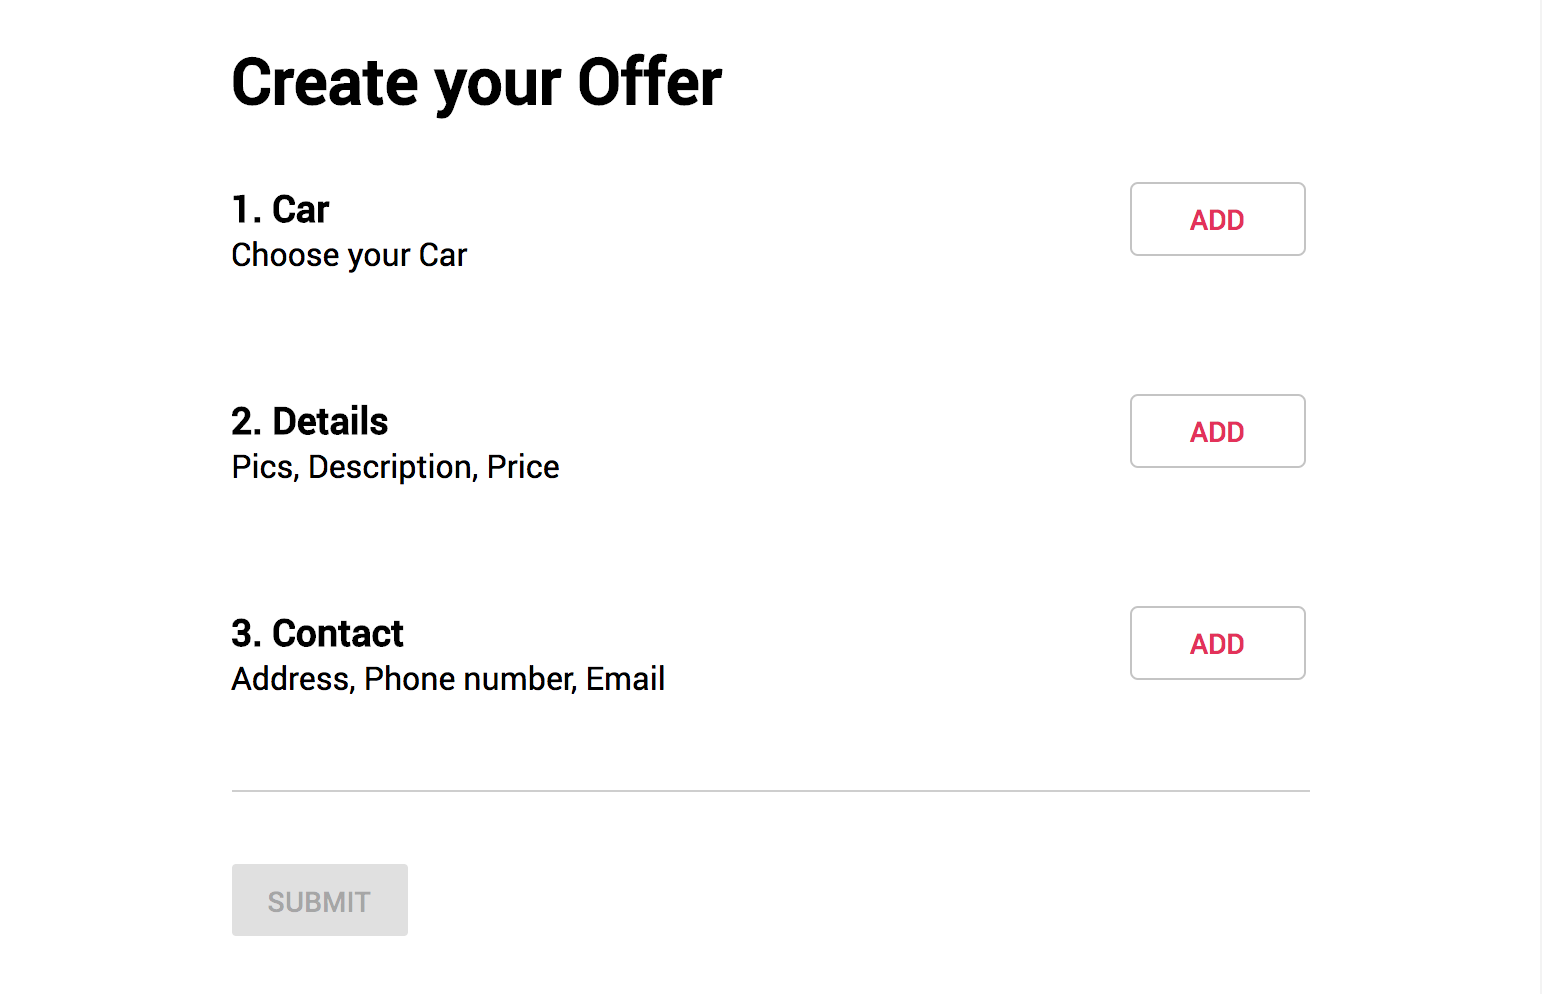
\includegraphics[width=1\textwidth]{figures/cryptoride_screens/create_offer.png}}
% \caption{Screen: Create Offer \label{fig:screen_create_offer}}
% \end{figure}
%
% \begin{figure}[htbp]
% \centerline{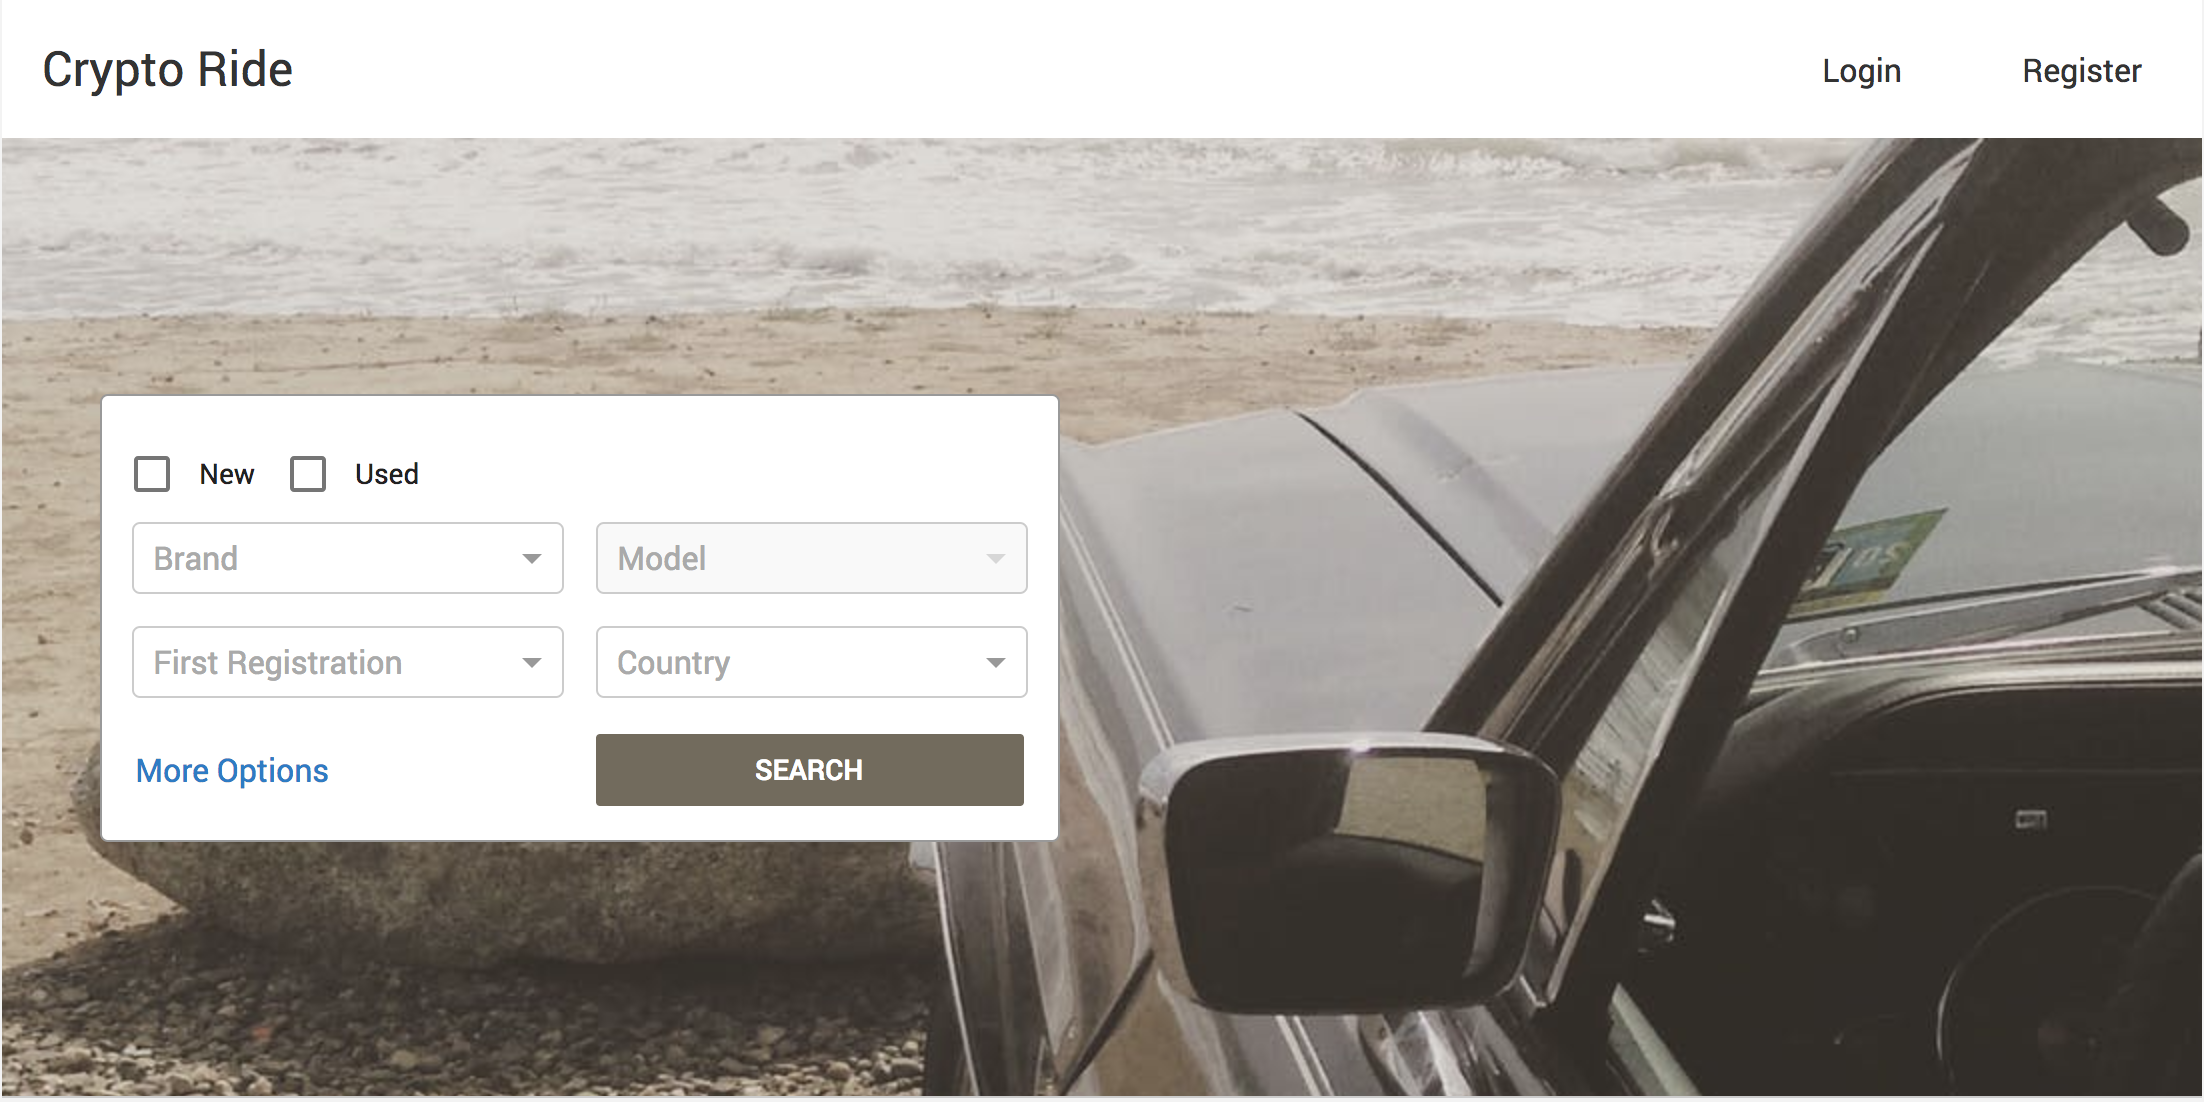
\includegraphics[width=1\textwidth]{figures/cryptoride_screens/cryptoride_landing_page.png}}
% \caption{Screen: Landing page \label{fig:screen_landing_page}}
% \end{figure}
%
%
% \begin{figure}[htbp]
% \centerline{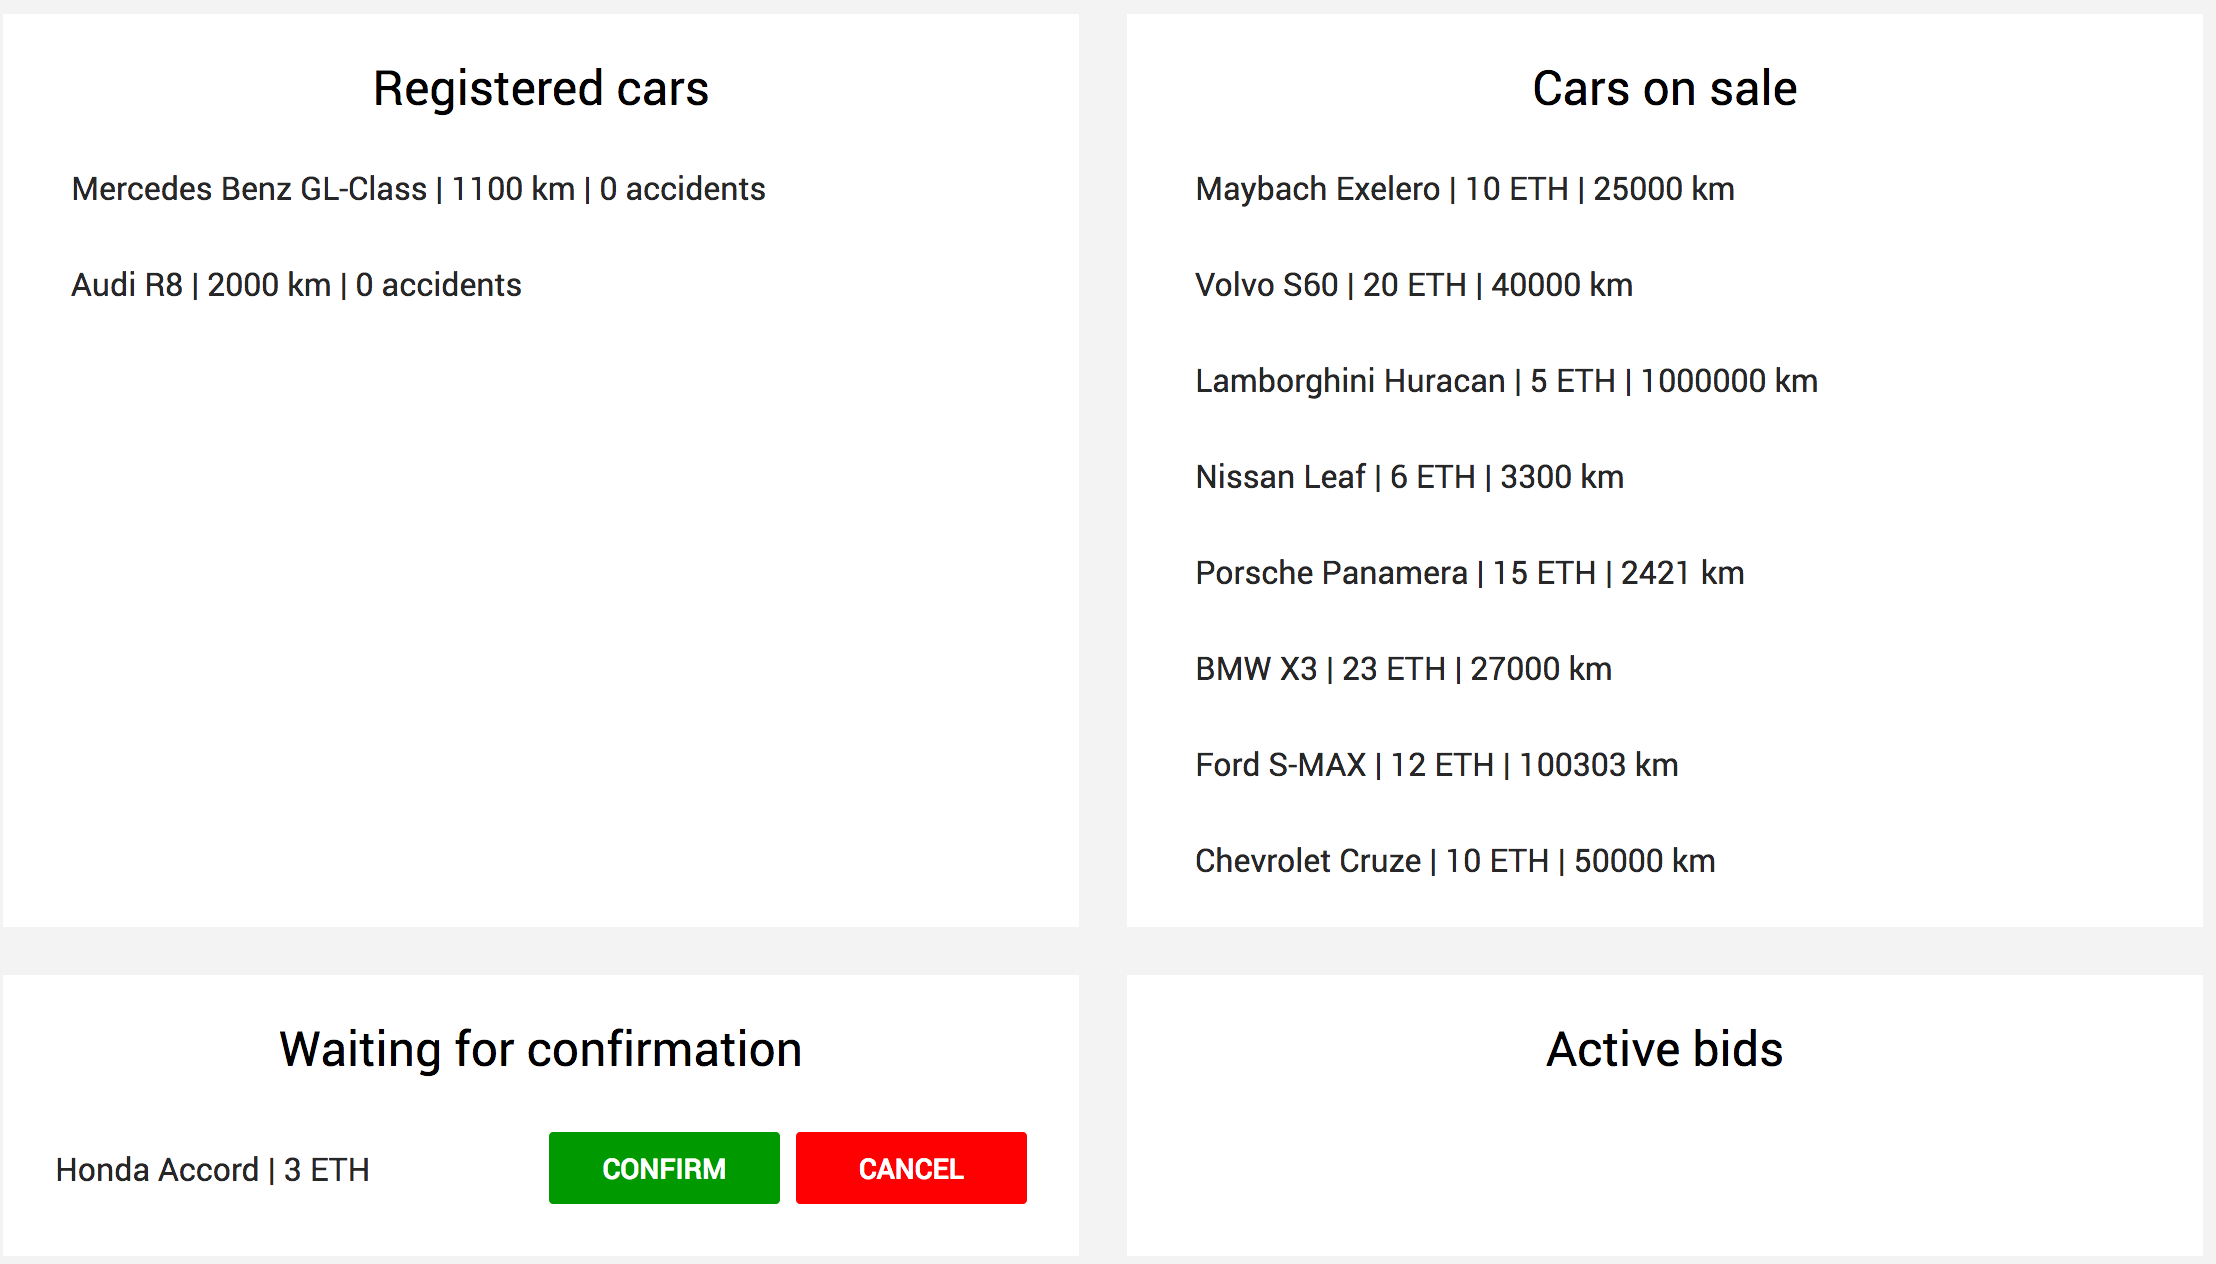
\includegraphics[width=1\textwidth]{figures/cryptoride_screens/my_cars.png}}
% \caption{Screen: My cars \label{fig:screen_my_cars}}
% \end{figure}
%
% \begin{figure}[htbp]
% \centerline{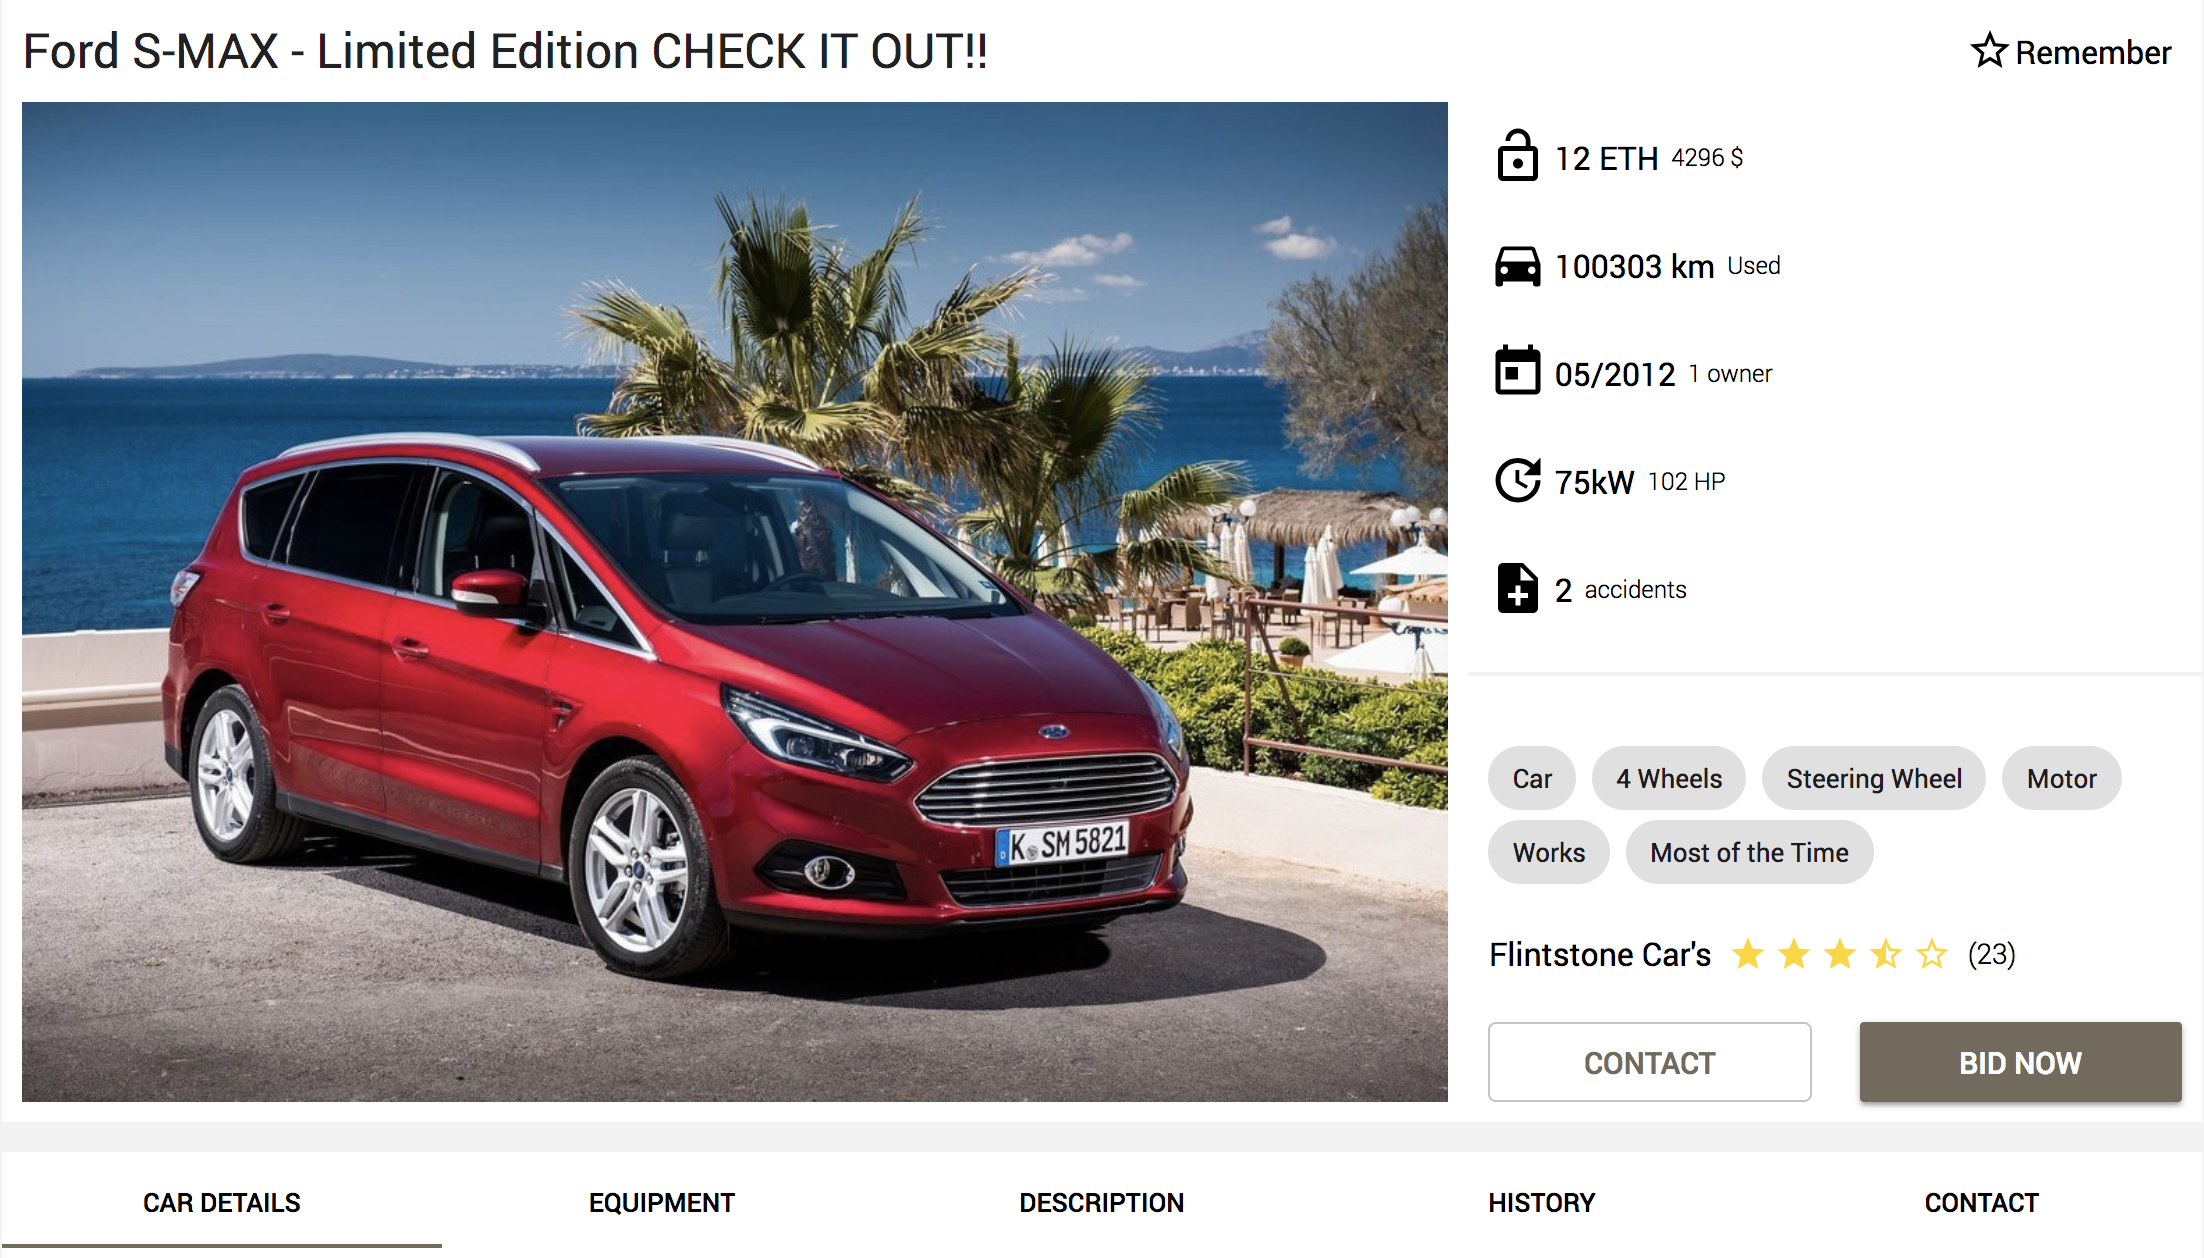
\includegraphics[width=1\textwidth]{figures/cryptoride_screens/offer_details.png}}
% \caption{Screen: Over details \label{fig:screen_offer_details}}
% \end{figure}
%
% \begin{figure}[htbp]
% \centerline{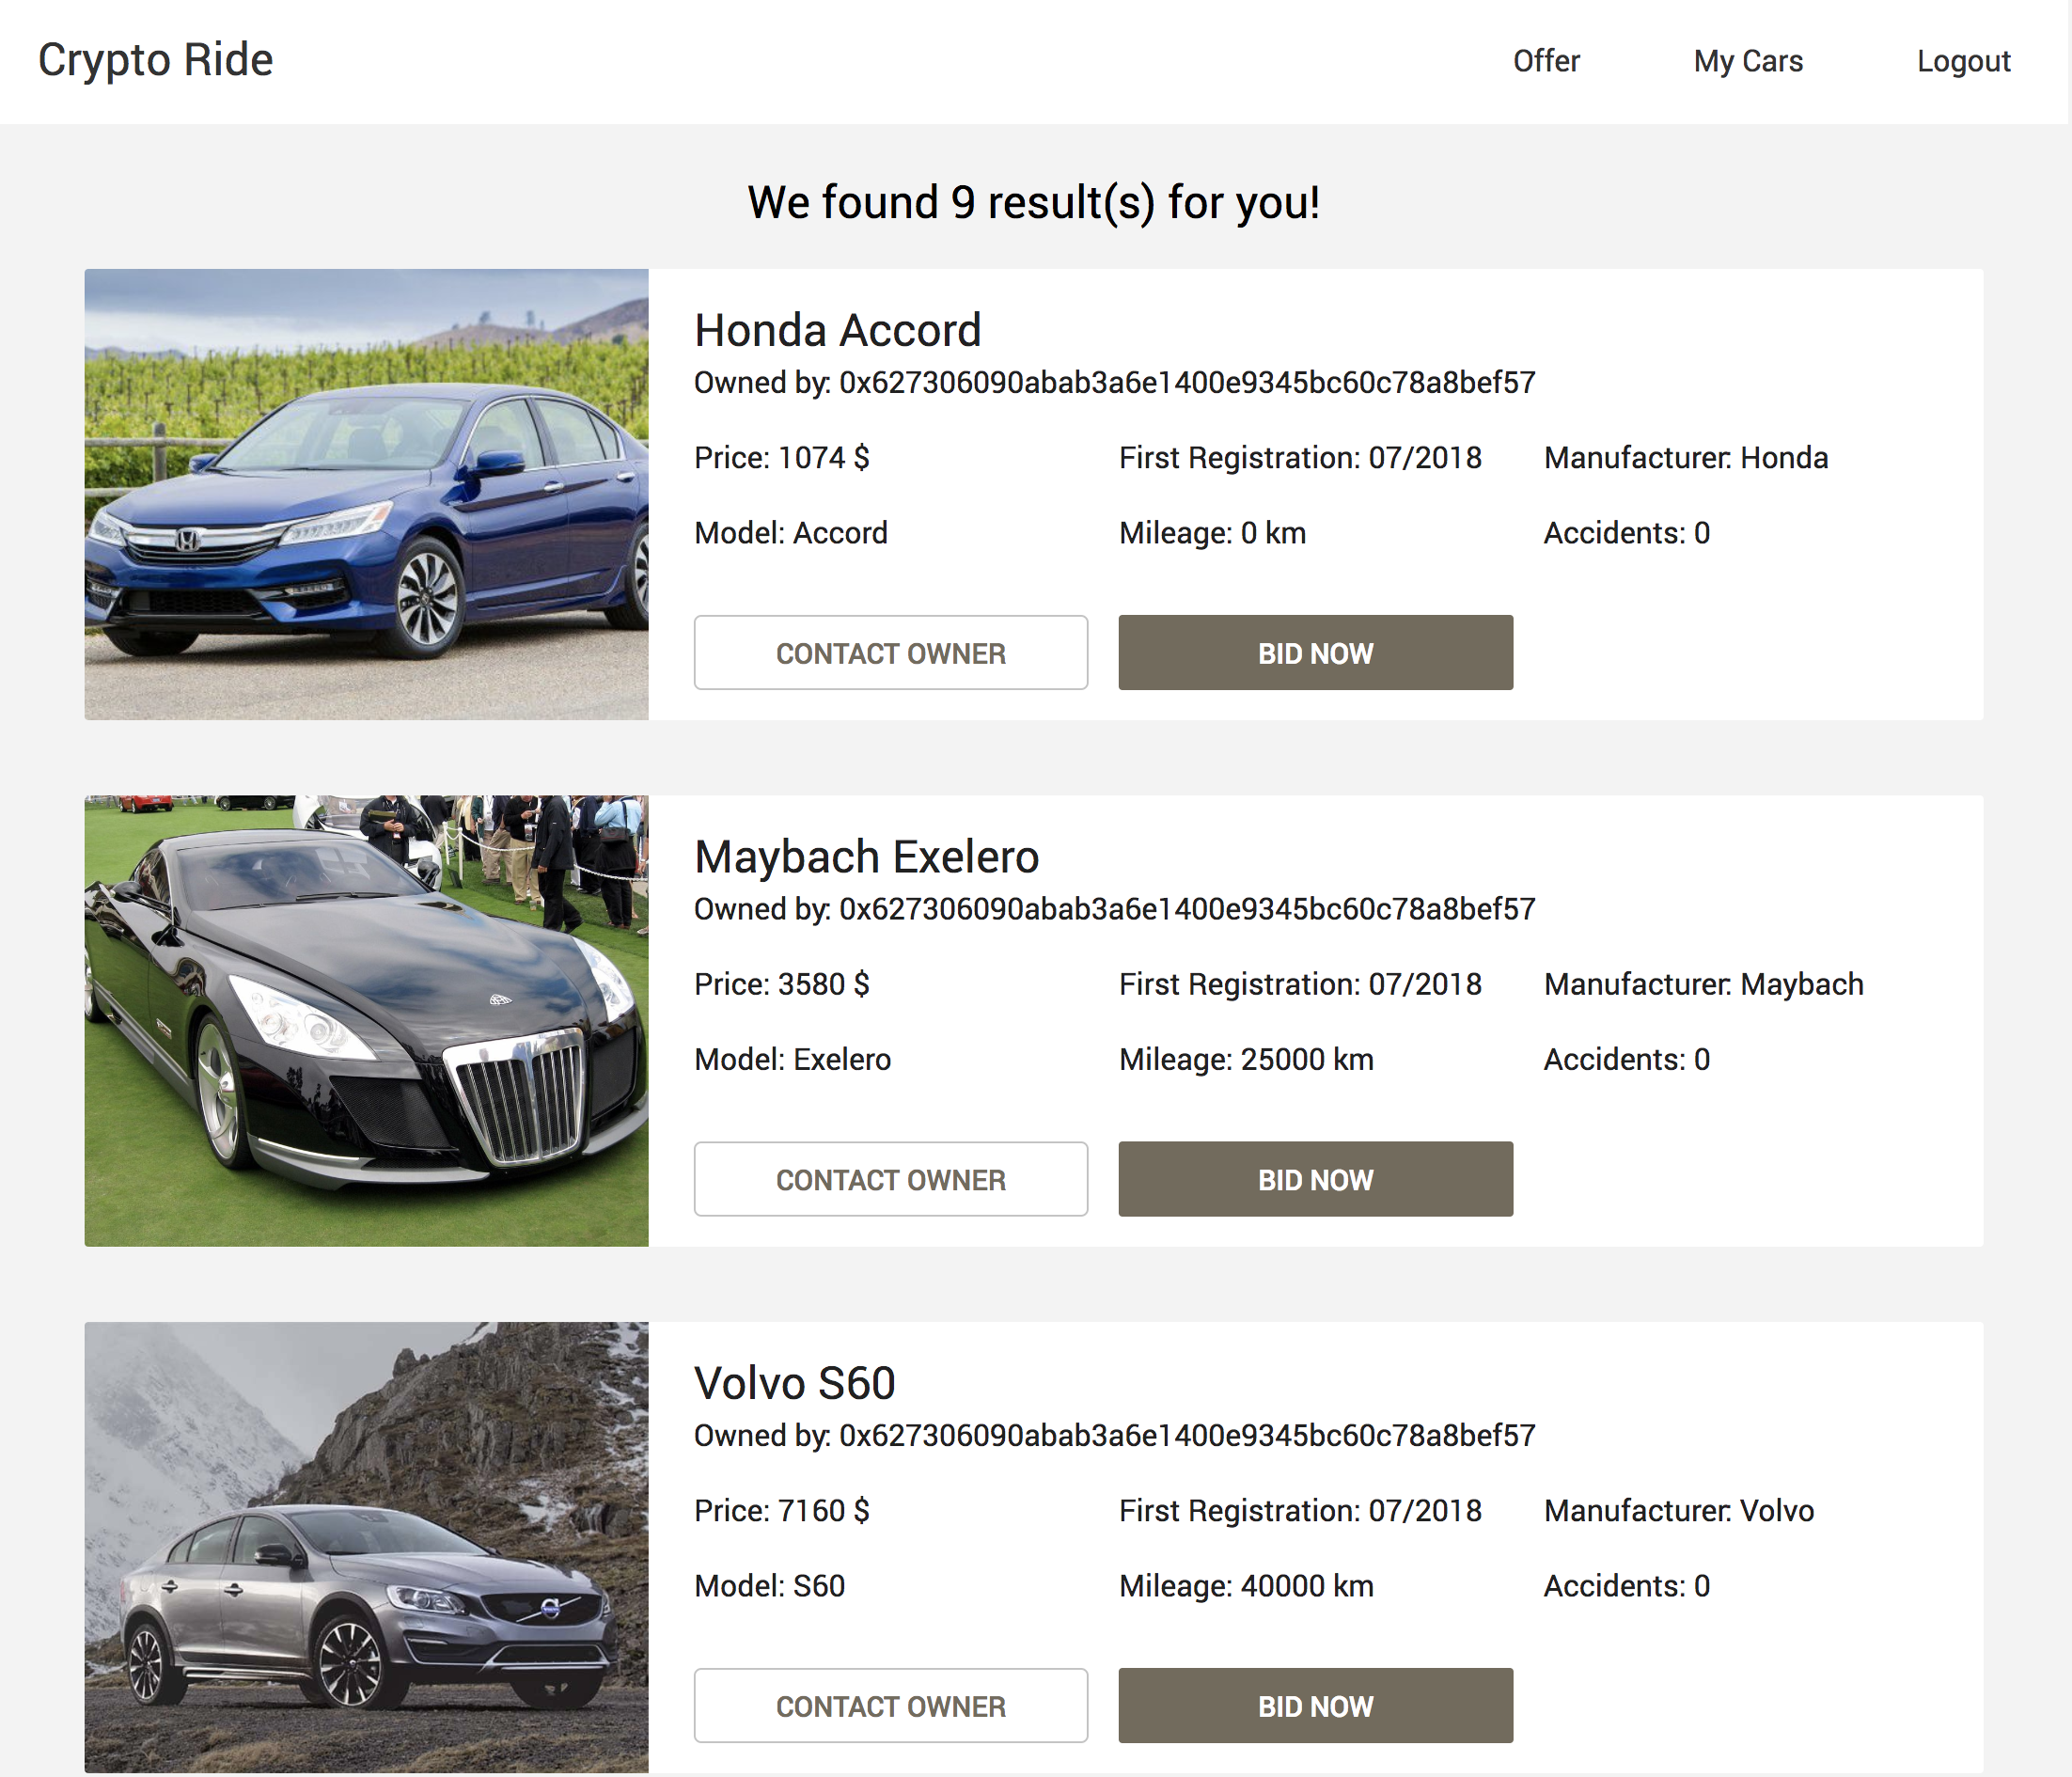
\includegraphics[width=1\textwidth]{figures/cryptoride_screens/offers_overview.png}}
% \caption{Screen: Overs overview \label{fig:screen_offers_overview}}
% \end{figure}
